\subsection{Lecture de courant}
	\paragraph*{}
	La lecture du courant est essentielle pour éviter que la batterie ne se charge ou se décharge excessivement. Cette information va aussi être utilisée pour l'estimation de l'état de charge, fonctionnalité qui va être implémentée après le cours ELE-791. Pour que l'estimation de charge soit précise sans accumuler une grande erreur, la lecture de courant se doit d'être la plus précise sur toute la plage d'utilisation. L'objectif est donc d'avoir une précision qui beaucoup plus grande que le 2\% des spécifications. 
	
	\paragraph*{}
	Eclipse IX utilise présentement la première technique. La résistance est cependant loin de la carte qui prend la mesure, ce qui pourrait causer certains problèmes étant donné que les deux fils ont des signaux avec de très faibles voltages qui sont lus par un amplificateur avec une impédance élevée. Afin d'avoir une lecture robuste et mieux protégée du bruit, le circuit de lecture de courant aura sa propre carte au lieu d'être sur la carte maître. Les longs fils auront ainsi la communication qui est beaucoup plus résistante aux bruits. 
	
	\paragraph*{}
	Deux différentes techniques ont été envisagées pour mesurer le courant. La première est de lire la tension aux bornes d'une résistance en série avec la batterie et la deuxième est d'utiliser un capteur à effet Hall. 
	
	
	\subsubsection*{Lecture de la tension aux bornes d'une résistance en série avec la batterie}
	\paragraph*{}
	Les résistances "shunt" ont une très grande précision ($\pm 0.1 \% , \pm 0.5 \%$), elles sont faciles à interfacer et faciles à remplacer lorsque les spécifications changent. Un amplificateur avec une grande impédance d'entrée est nécessaire pour amener le signal analogique de très faible amplitude entre 0V et le voltage de référence de l'ADC. L'amplificateur doit avoir un gain très précis, être thermiquement stable et avoir une bonne atténuation du bruit en mode commun. Le bruit en mode commun peut être réduit en ayant le circuit de lecture référencé à la borne négative de la batterie et en plaçant la résistance en série avec cette même borne.
		
	\paragraph*{}
	Pour avoir une bonne lecture avec un minimum de bruit, une configuration avec l'amplificateur avec une sortie différentiel connecté à un ADC avec une entrée différentielle serait la plus robuste et précise puisque le signal sera au-dessus du bruit de fond (noise floor). L'amplificateur PGA281 et le convertisseur analogue à numérique ADC141S626 de Texas Instrument possèdent les différentes caractéristiques recherchées. La résistance de 250 $\mu \Omega$ d'Éclipse IX serait réutilisée pour Éclipse X.
	
	\begin{figure}[H]
		\centering
		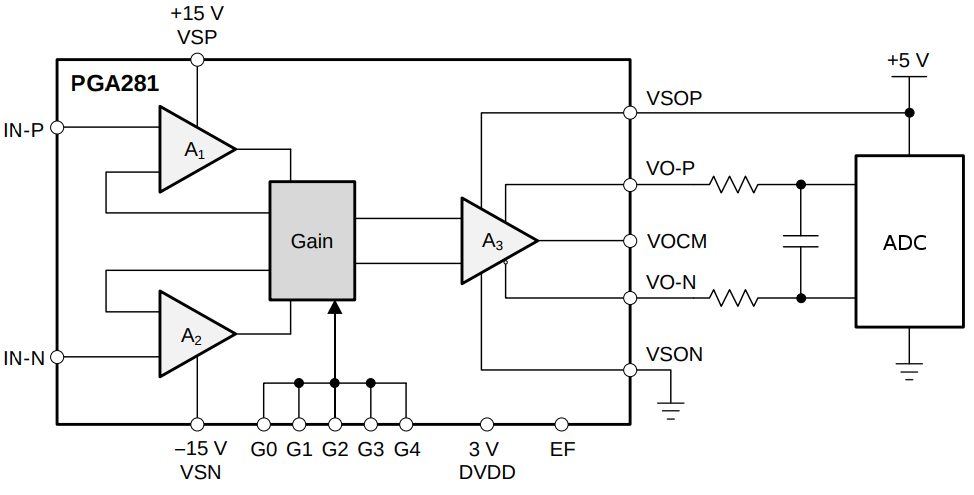
\includegraphics[scale = 0.4]{Images/current_sense_shunt.png}
		\caption{Configuration de l'amplificateur et de l'ADC.}
		\label{fig:current_sense_shunt}
	\end{figure}
	
	\subsubsection*{Senseur à effet Hall}
	\paragraph*{}	
	Un capteur à effet Hall à l'avantage de ne pas être intrusif et d'être isolé. Les senseurs ratio métrique en boucle ouverte ont une bonne précision qui correspond aux spécifications, il ne sont pas dispendieux et ils sont très faciles à interfacer. Le HO 100-S de LEM n'a pas besoin d'amplificateur et peut ainsi être branché directement sur l'entrée du ADC. Les effets Hall ont besoin de calibration pour éliminer le décalage lorsqu'il n'y a aucun courant. Ces senseurs ont aussi le désavantage d'avoir certaines non-linéarités dans le gain et une hystérésis. Une bonne caractérisation et calibration du senseur réduirait grandement ces inconvénients.
	
	\subsubsection*{Choix final}
	\paragraph*{}
	Le courant sera lu en utilisant la résistance en série avec la borne négative de la batterie. Sa flexibilité, sa robustesse et l'absence de calibration en font la solution la plus facile à implémenter tout en étant plus sûre de respecter les spécifications. Il serait cependant intéressant dans le futur de faire une carte avec le capteur à effet Hall pour avoir une mesure redondante et comparer les deux solutions dans la voiture.	
		